\section{Data Types}
In the computer data are all binary digits (actually 0 and +5 volts).  At a higher level of abstraction data are typed into integers, real, or alphanumeric representation.  The type affects the kind of arithmetic operations that are allowed (as well as the kind of arithmetic -- integer versus real arithmetic; lexicographical ordering of alphanumeric , etc.)

In scientific programming, a common (and really difficult to detect) source of slight inaccuracies (that tend to snowball as the program runs) is mixed mode arithmetic required because two numeric values are of different types (integer and real).

\subsection{Integer}
Integers are numbers without any fractional portion (nothing after the decimal point -- which is not used in integers).  Numbers like -3, -2, -1, 0, 1, 2, 200 are integers.   A number like 1.1 is not an integer, and 1.0 is also not an integer (the presence of the decimal point makes the number a real).

To declare an integer in Python, just assign the variable name to an integer for example
\begin{verbatim}
MyPhoneNumber = 14158576309  
\end{verbatim}

\subsection{Real (Float)}
A real or float is a number that has (or can have) a fractional portion -- the number has decimal parts. The numbers 3.14159, -0.001, 11.11, 1., are all floats.   The last one is especially tricky, if you don't notice the decimal point you might think it is an integer but the inclusion of the decimal point in Python tells the program that the value is to be treated as a float.

To declare a float in Python, just assign the variable name to a float for example
\begin{verbatim}
MyMassInKilos = 74.8427
\end{verbatim}

\subsection{String (Alphanumeric)}
A string is a data type that is treated as text elements.  The usual letters are strings, but numbers can be included.  The numbers in a string are simply characters and cannot be directly used in arithmetic.  There are some kinds of arithmetic that can be performed on strings but generally we process string variables to capture the text nature of their contents.

To declare a string in Python, just assign the variable name to a string value -- the trick is the value is enclosed in quotes.  The quotes are delimiters that tell the program that the characters between the quotes are characters and are to be treated as literal representation.  For example
\begin{verbatim}
MyName = 'Theodore'
MyCatName = "Dusty"
DustyMassInKilos = "7.48427"
\end{verbatim}
are all string variables.  The last assignment is made a string on purpose.   String variables can be combined using an operation called concatenation.   The symbol for concatenation is the plus symbol \texttt{+}.  

Strings can also be converted to all upper case using the \texttt{upper()} function.   The syntax for the \texttt{upper()} function is \texttt{'string to be upper case'.upper()}.   Notice the ``dot'' in the syntax.   The operation passes everything to the left of the dot to the function which then operates on that content and returns the result all upper case (or an error if the input stream is not a string).

\begin{figure}[h!] %  figure placement: here, top, bottom, or page
   \centering
   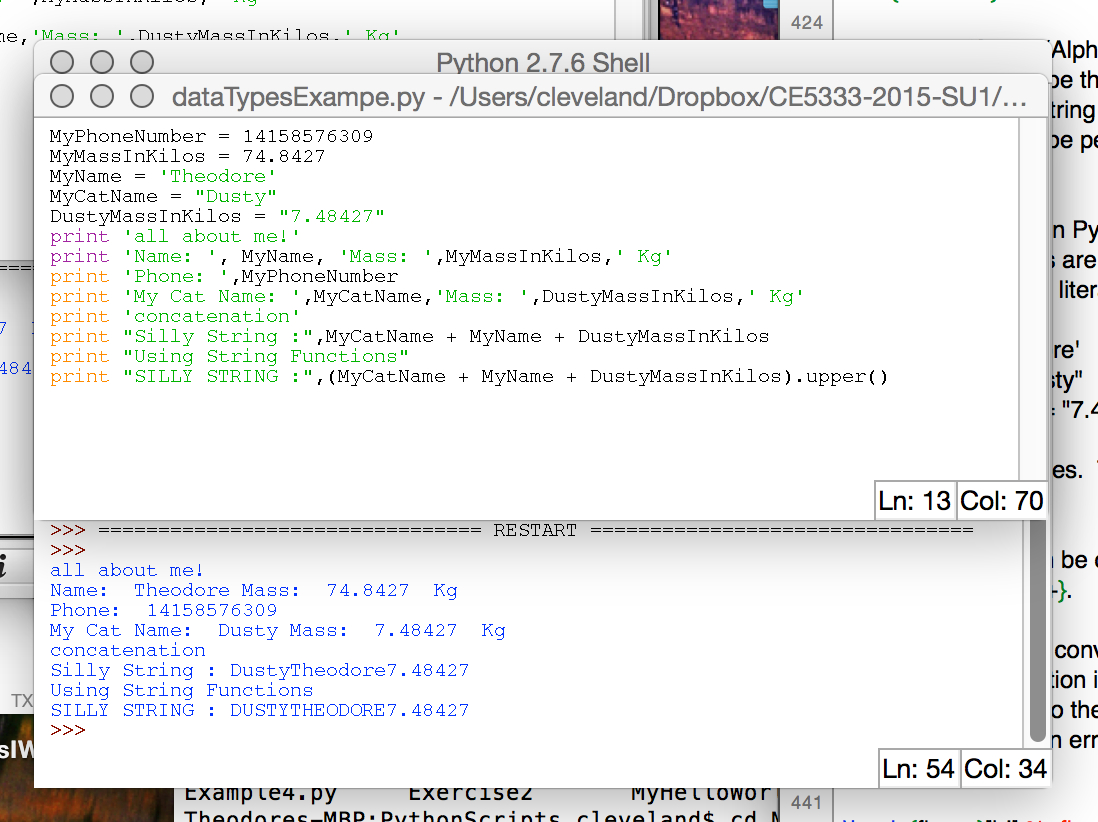
\includegraphics[width=5in]{./4-DataTypes/DataTypesExample.jpg} 
   \caption{Examples of data types and their appearance when printed}
   \label{fig:DataTypesExample}
\end{figure}

Figure \ref{fig:DataTypesExample} is a screen capture of the various assignments so far.  Notice how Dusty's mass appears to be a number, but in reality it is a string variable -- if it were used in arithmetic it would cause an error.

\subsubsection{Formatting Strings}
Strings can be formatted using the \texttt{\%} operator or the \texttt{format()} function.  The concepts will be introduced later on as needed in the workbook, you can Google search for examples of how to do such formatting.  My personal preference would be with the \texttt{format()} function because it is clear what is going on, whereas the \texttt{\%} operator I find hard to interpret when I am maintaining code.   

\subsection{Changing Types}
A variable type can be changed.  This activity is called type casting.  Three functions allow type casting: \texttt{int()}, \texttt{float()}, and \texttt{str()}.
The function names indicate the result of using the function, hence \texttt{int()} returns an integer, \texttt{float()} returns a float, and \texttt{str()} returns a string.

\begin{figure}[h!] %  figure placement: here, top, bottom, or page
   \centering
   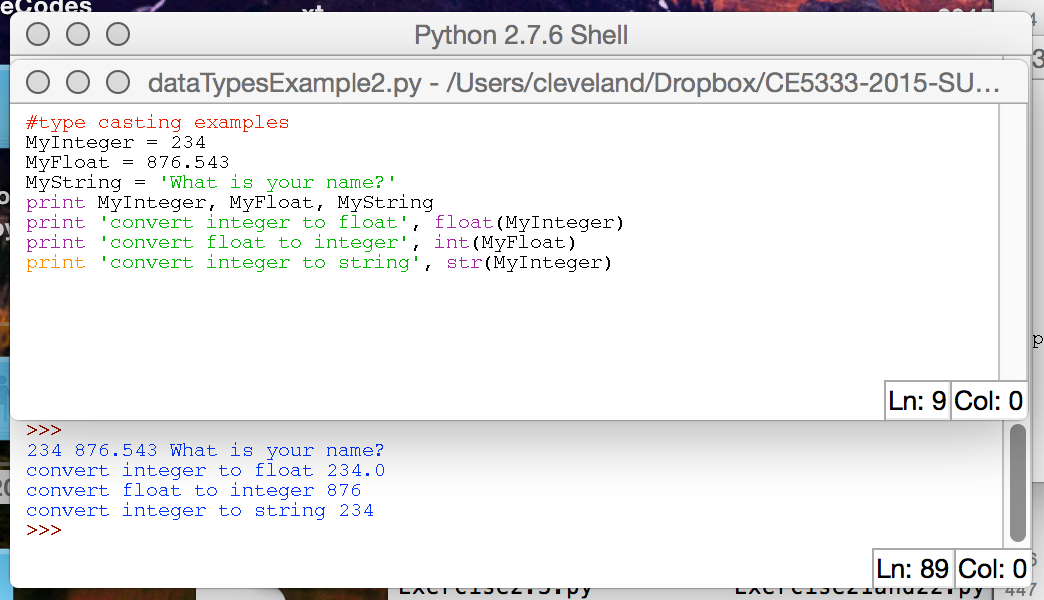
\includegraphics[width=5in]{./4-DataTypes/DataTypesExample2.jpg} 
   \caption{Converting data types}
   \label{fig:DataTypesExample2}
\end{figure}
The easiest way to understand is to see an example.  Figure \ref{fig:DataTypesExample2} is a screen capture illustrating some type casting.   We cannot convert arbitrary strings (with letters) into numeric variables using the functions as-is, there would be some coding involved. 
\subsection{List (Array)}
A list is a collection of data that are somehow related.  It is a convenient way to refer to a collection of similar things by a single name, and using an index (like a subscript in math) to identify a particular item.

Consider the ``math-like'' variable $x$ below:\\
~\\
\begin{math}
x_0 = 7 \\
x_1 = 11\\
x_2 = 5\\
x_3 = 9\\
x_4 = 13\\
\dots \\
x_N = 223\\
\end{math}\\
The variable name is $x$ and the subscripts correspond to different values.   Thus the \textbf{value} of the variable \textbf{named} $x$ associated with \textbf{subscript} $3$ is the number $9$.

\begin{figure}[h!] %  figure placement: here, top, bottom, or page
   \centering
   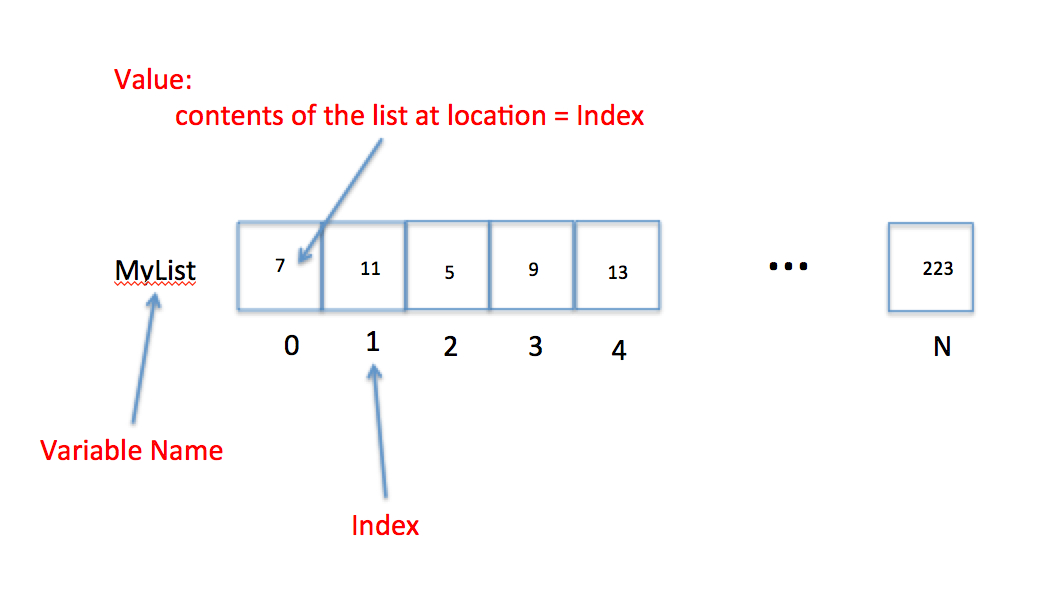
\includegraphics[width=5in]{./4-DataTypes/ListConcept.jpg} 
   \caption{Visual schematic of the list concept}
   \label{fig:ListConcept}
\end{figure}

Figure \ref{fig:ListConcept} is a visual representation of the concept that treats a variable as a collection of cells.  In the figure, the variable \textbf{name} is \textsl{MyList}\footnote{Ok that's a silly name, but I wanted something different than $x$.}, the subscripts are replaced by an \textsl{index} which identifies which cell is being referenced.  The \textbf{value} is the cell content at the particular \textbf{index}.   So in the figure the \textbf{value} of \textbf{MyList} at \textbf{Index} = 3 is the number $9$.

In scientific programming we use lists a lot -- we usually call then vectors, arrays, matrices and such, but they are ultimately just lists.

To declare a list you can write the list name and assign it values.  The square brackets are used to identify that the variable is a list.  Like:
\begin{verbatim}
MyList = [7,11,5,9,13,66,99,223]
\end{verbatim}

One can also declare a null list and use the \texttt{append()} method to fill it as needed.   
\begin{verbatim}
MyOtherList = [ ]
\end{verbatim}

Ok in Python, indices always start at \textbf{ZERO}.  I find this to be a source of confusion because my first language was FORTRAN at that language started counting at ONE.  Otherwise its just the convention.  The first element in a list has an index of 0, the second an index of 1, and so on.

We access the contents of a list by referring to its name and index.  For example
\texttt{MyList[3]} has a value of the number $9$.



\begin{figure}[h!] %  figure placement: here, top, bottom, or page
   \centering
   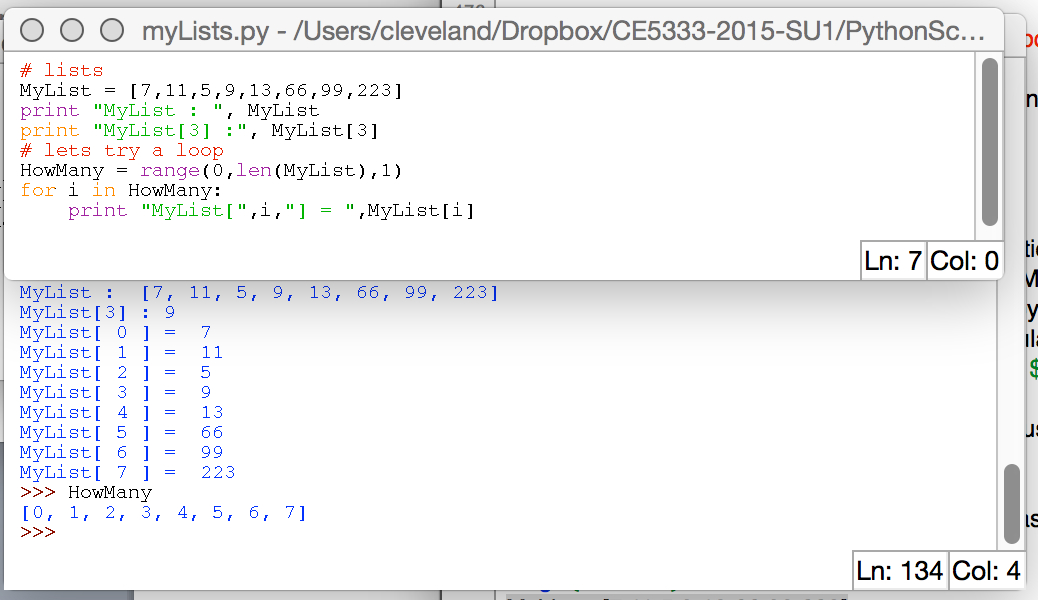
\includegraphics[width=5in]{./4-DataTypes/ListExample.jpg} 
   \caption{Example of list creation, addressing, and contents.  Also introduces the \texttt{range()} function.}
   \label{fig:ListExample}
\end{figure}

Figure \ref{fig:ListExample} is a screen capture showing some of these list operations.  The example creates \texttt{MyList} then prints its contents.  That shows as the list printed across the line.   Then the 4th element (index == 3) is printed.   Lastly a special kind of list is built using the \texttt{range(start,end,step)} function.  This function returns a list of numbers that starts at ``start'', ends at ``end'', and increments in units of ``step.''   The result is assigned to a variable named \texttt{HowMany} and this variable is itself just a list.   We could have put the range function directly into the ``for'' loop -- but it makes the parts of the example harder to keep track of.

We have seen a ``for'' loop earlier in an exercise.   Scientific programming uses loops a lot (in fact most programming uses loops -- the benefit of a computer is the ability for it do do stuff over and over again -- this is called iteration (or repetition)).  There are tricks to doing loops fast -- thats for another time.

\subsubsection{Special List -- Tuple}
A tuple is a special kind of list where the values cannot be changed after the list is created.  It is useful for list-like things that are static -- like days in a week, or months of a year.

You declare a tuple like a list, except use round brackets instead of square brackets\footnote{Here the declaration is broken across two lines to fit the page -- it is a single line IDLE}.  
\begin{verbatim}
MyTupleName = ("Jan","Feb","Mar","Apr","May","Jun",
                        "Jul","Aug","Sep","Oct","Nov","Dec")
\end{verbatim}

\subsubsection{Special List -- Dictionary}
A dictionary is a special kind of list where the items are related data PAIRS.  It is a lot like a relational database (it probably is one in fact) where the first item in the pair is called the key, and must be unique in a dictionary, and the second item in the pair is the data.   The second item could itself be a list, so a dictionary would be a meaningful way to build a database in Python.

To declare a dictionary using curly brackets
\begin{verbatim}
MyPetsNamesAndMass = { "Dusty":7.8 , "Aspen":6.3, "Merrimee":0.03}
\end{verbatim}

To declare a dictionary using the \texttt{dict()} method
\begin{verbatim}
MyPetsNamesAndMassToo = dict(Dusty = 7.8 , Aspen = 6.3, Merrimee = 0.03)
\end{verbatim}

Figure \ref{fig:TuplesAndDicts} shows some examples of a Tuple and Dictionary constructs.   The last row in the program is an attempt to clobber the contents of a Tuple and the related error message.

\begin{figure}[h!] %  figure placement: here, top, bottom, or page
   \centering
   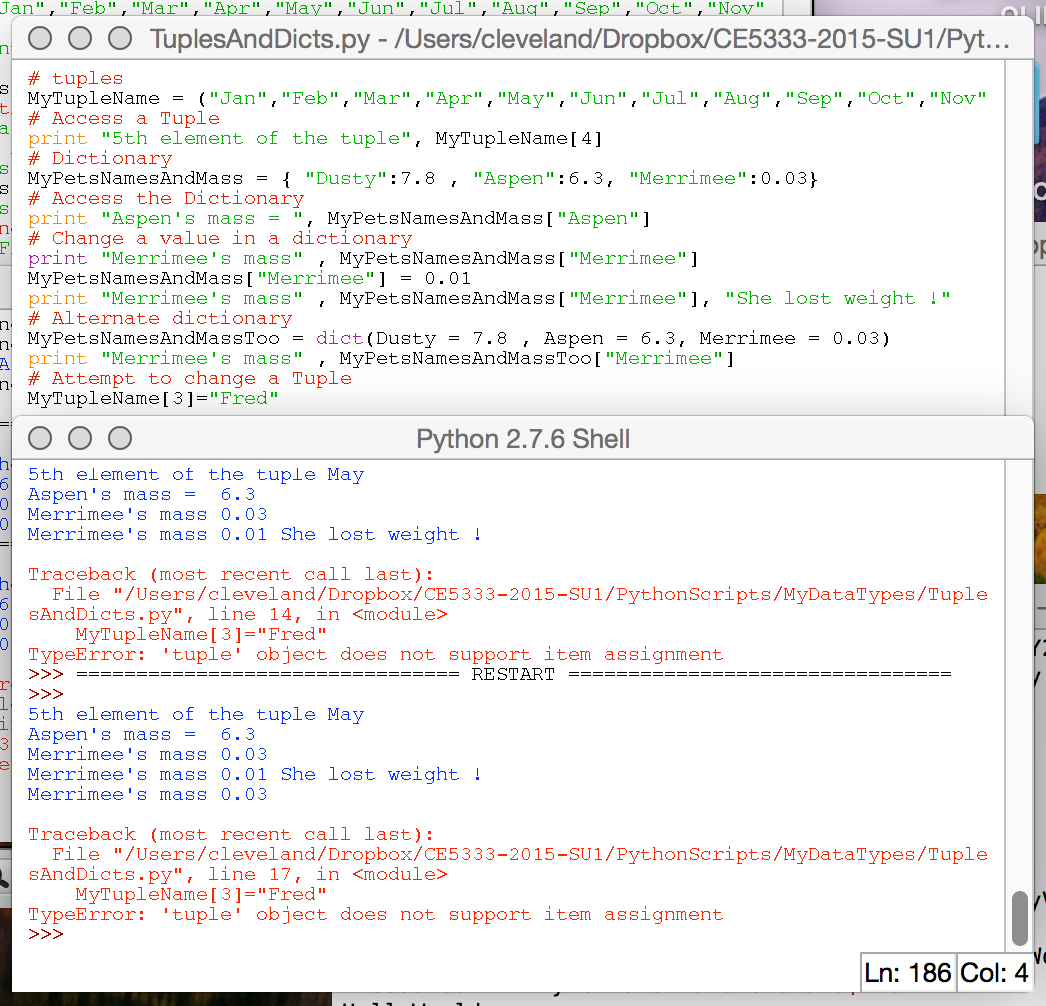
\includegraphics[width=5in]{./4-DataTypes/TuplesAndDicts.jpg} 
   \caption{A Tuple and a Dictionary}
   \label{fig:TuplesAndDicts}
\end{figure}
\clearpage
\subsection{Getting data into a program -- the \texttt{input()} function}
I am finishing this section with introduction to the \texttt{input()} function so that we can start some meaningful exercises.  

The input function has the following structure it looks like \\
\texttt{ MyVariable = input("Message to prompt input")}

\begin{figure}[h!] %  figure placement: here, top, bottom, or page
   \centering
   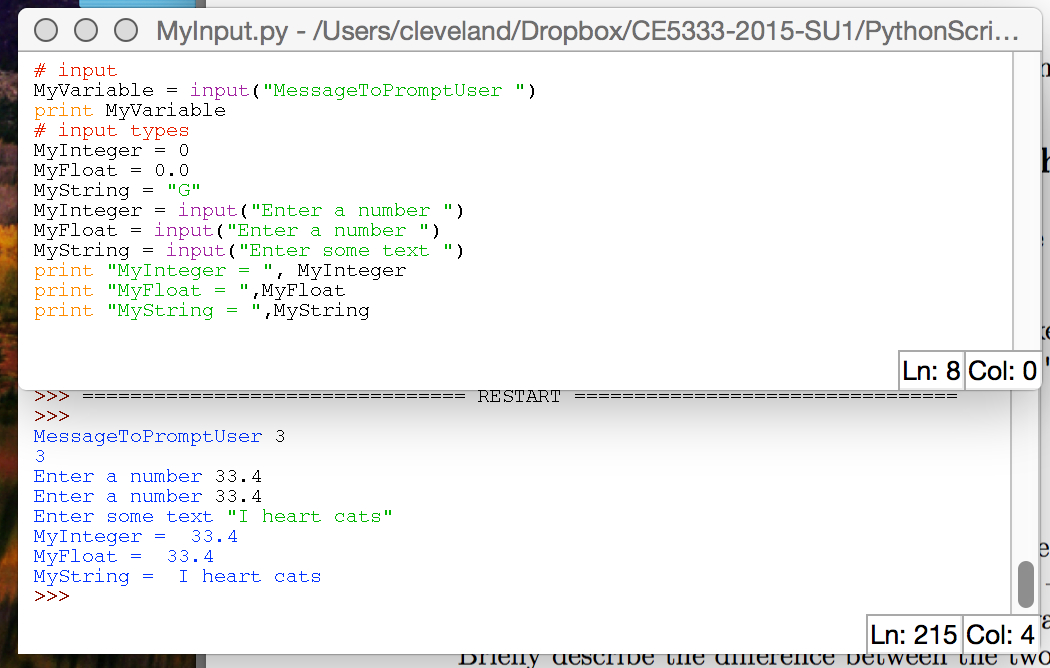
\includegraphics[width=6in]{./4-DataTypes/SimpleInputs.jpg} 
   \caption{Using the \texttt{input()} function.}
   \label{fig:SimpleInputs}
\end{figure}

Figure \ref{fig:SimpleInputs} is an example of using the \texttt{input()} function for very simplistic input.  Later on when we learn about formatted strings for the message body, much more complicated input can be used.   Notice how the input function clobbered our integer variable and wrote the value to the variable as type == float.  As presented here the input function will read the input stream and make a guess as to the data type and assign that to the destination variable, clobbering the existing variable type if necessary.

\clearpage
\subsection{Exercises}
\begin{enumerate}
%\item Use Google search and learn about the difference between integer and floating arithmetic.  You can get lost in a internet vortex -- you will want to avoid the computer hardware kind of links (you will know right away when there are images of logic gates).   Briefly describe the difference between the two types of arithmetic.

\item Create a new file in the IDLE editor and type in the code below.  Save and run the script.
\begin{verbatim}
# data types
print 'integers and reals'
x1 = 1.0
y1 = 1.
z1 = 1
x2 = 5.0
y2 = 5.
z2 = 5
print 'x1 = ', x1, ' y1 = ', y1, ' z1 = ', z1
print 'x2 = ', x2, ' y2 = ', y2, ' z2 = ', z2
print 'x1/x2 = ',x1/x2,' y1/y2 = ',y1/y2,' z1/z2 = ',z1/z2
\end{verbatim}
\begin{enumerate} 
 \item Of the six variables, which are integers?
 \item What is the difference (in effect) between \texttt{x1=1.0} and \texttt{y1=1.}?
 \item Examine the division results; Why does \texttt{z1/z2} return a value of \texttt{0}?
\end{enumerate}

\item Create a new file in the IDLE editor and consider the mathematical list below.  Using the for loop example, we can have the program square each element in the list and place that result in a second list.\\
~\\
\begin{math}
x_0 = -1 ~~~ x_1 = 0 ~~~ x_2 = 1 ~~~ x_3 = 2\\
\end{math}\\
\begin{verbatim}
# list of squares
x = [-1,0,1,2]
y = [0,0,0,0]
HowMany = range(0,len(x),1)
for i in HowMany:
    y[i]=x[i]**2
print "x: ",x
print "y: ",y
\end{verbatim}

Type in the code above and verify that indeed it returns in the list named ``y'' the square of each element in ``x.''  Now modify the code to do the same exercise except with the list of six elements
~\\
\begin{math}
x_0 = -1 ~~~ x_1 = 0 ~~~ x_2 = 1 ~~~ x_3 = 2 ~~~ x_4 = 3 ~~~ x_5 = 4\\
\end{math}\\

The script is hardly elegant but functions OK.
\begin{enumerate}
\item Why is the variable ``y'' declared as a list of zeros instead of a null list?
\item Employ a different way to build ``y'' so the programmer doesn't have to modify both lists for the longer mathematical list. (Hint: at least one other way is kind of hidden in plain sight in the code itself!)
\end{enumerate}

\item Use the input function to write a script that asks the user for a number, and returns the cube of the number.

\end{enumerate}


%%%%%%%%%%%%%%%%%%%%%%%%%%%%%%%%%%%%%%%%%%%%%%%%%%%%%%%%%%%%%%%
